\subsubsection{Elevator}

\begin{enumerate*}

  \item The current module was divided into 3 submodules. Next, there were composed technical specifications for each submodule:
  \begin{enumerate*}
  	\item Lifting mechanism
  	\begin{enumerate*}
  		\item The lifting mechanism will be used to deliver the bucket for debris to the second and the top goal and the hooks for grasping to the pullup bar.
  		
  		\item The lift should be telescopic. It should have two guides that move along parallel lines. Each guide should consist of a cascade of segments which do not exceed the start cube but can be extracted after the match starts.
  		
  		\item The guides should be extracted by the cables (one cable for a guide). When the cables are pulled by the reeling mechanism, the guides are going up. The full extracting should take no more than 4 seconds.
  		
  		\item  The length of the guides should be enough to perform it's tasks.
  		
  	\end{enumerate*}
  	
  	\item Turning mechanism
  	\begin{enumerate*}
  		\item The turning mechanism will be used to vary the angle of tilt of the lifting mechanism. It is demanded to provide the robot with two positions of elevator: in the first position it exstracts so that we can through debris to the top box from the low zone, in the second psition the angle of incline allows us to grasp the pullup bar from the second zone.
  		
  		\item The turning mechanism should be powered by a continuous rotation servo to save DC motors.
  		
  		\item It should be used a worm gear on the shaft of the servo to provide one-direction force and prevent the platform with reeling mechanism to move itself.
  		
  	\end{enumerate*}
  	
  	\item Reeling mechanism (winch)
  	\begin{enumerate*}
  		\item The main option of the reeling mechanism is extracting of the lifting mechanism. The second option, that can be realised with it is the pulling up.
  		
  		\item The reeling mechanism should consist of two coils for reeling the cables from guides. Using distinct coils will help to avoid the entanglement of the cables. However, both coils can be mounted to one axis. Coils can be powered by 2-4 DC motors.
  		
  		\item To provide the pulling up there are needed two additional coils for reeling the strong cables. The principle of work is folowing: when the first pair of coils pulls the cable and extracts the elevator, the another pair of coils releases strong cables used for pulling up. When the elevator is fully put forward, so does the pull-up cable. Next, when all the coils rotate backwards, they pull the pull-up cable and release lifting mechanism's cables causing it to fold back.
  		
  		\item Two cables are needed to provide the steady pulling up. The strong cables should detach from the lifting mechanism after the hooks will be put to the bar to prevent damage of the elevator.
  		
  	\end{enumerate*}
  	
  \end{enumerate*}

  \item Next, it was started the designing of the robot.

  \begin{enumerate*}
    \item Lifting mechanism
    \begin{enumerate*}
       \item According to the technical plan our team created beforehand, the lifting mechanism was to consist of several construction beams connected to each other with special parts. To create these parts, we first thought through the concept and 3d-modeled them in Creo Parameteric 3.0. These parts are something akin to a brace and will stabilize one beam in relation to another. There are two types of braces: for the central gaps, and side gaps of the beams. Let us consider the simplest way to connect the two beams with these braces. Beam A will be fixed in place to the base of the robot, and beam B will be fixed relative to beam A. Then we can can connect the first three braces to the top of beam A and the second three braces to the bottom of beam B, allowing for maximum freedom of movement for one of the beams against the other. For greater stability we use two groups of three on each end of the beams.

       \item We must find such a height and length of the lifting mechanism that there would be an angle of tilt that would allow the robot to throw debris into the highest and middle bucket goals from the low zone, and grab the pull-up bar from the middle zone.

       \item Knowing that the individual beams are 350mm long, we calculated that in order to reach this height, we need four beams.

       \item Lifting four beams requires a block system - e.g. we need to add blocks with twine that, when reeled in, would lift the system.

       \item In order to fasten the braces we need to add caps on the end faces of the beams. I came to the conclusion that I needed to change the caps: drill a hole through their legs, so that the twine could be put through them, and grind off the heads somewhat in order to make a trough, through which to pass the line. This allowed me to avoid adding additional blocks on the beams.
    \end{enumerate*}
    \item Turning mechanism
    \begin{enumerate*}
       \item The turning mechanism consists of a servomotor attached to the base of the robot, a worm on the axis, and a gear on the first beam of the lifting mechanism. The servomotor turns the worm, which, in turn, rotates the gear, and the lifting mechanism tilts.
    \end{enumerate*}

    \item Reeling mechanism (winch)
    \begin{enumerate*}
    	\item The reeling mechanism is a system of two coils powered by 2-4 motors. It is both used for extracting elevator and pulling up. The principle of work is folowing: one coil pulls the cable and extracts the elevator when the another coil releases strong cable used for pulling up. When the elevator is fully put forward, so does the pullup cable. Next, when the coil rotates backwards, it pulls the pullup cable and releases elevator's cable causing it to fold back.
    \end{enumerate*}

  \end{enumerate*}	

  \begin{figure}[H]
  	\begin{minipage}[h]{0.31\linewidth}
  		\center{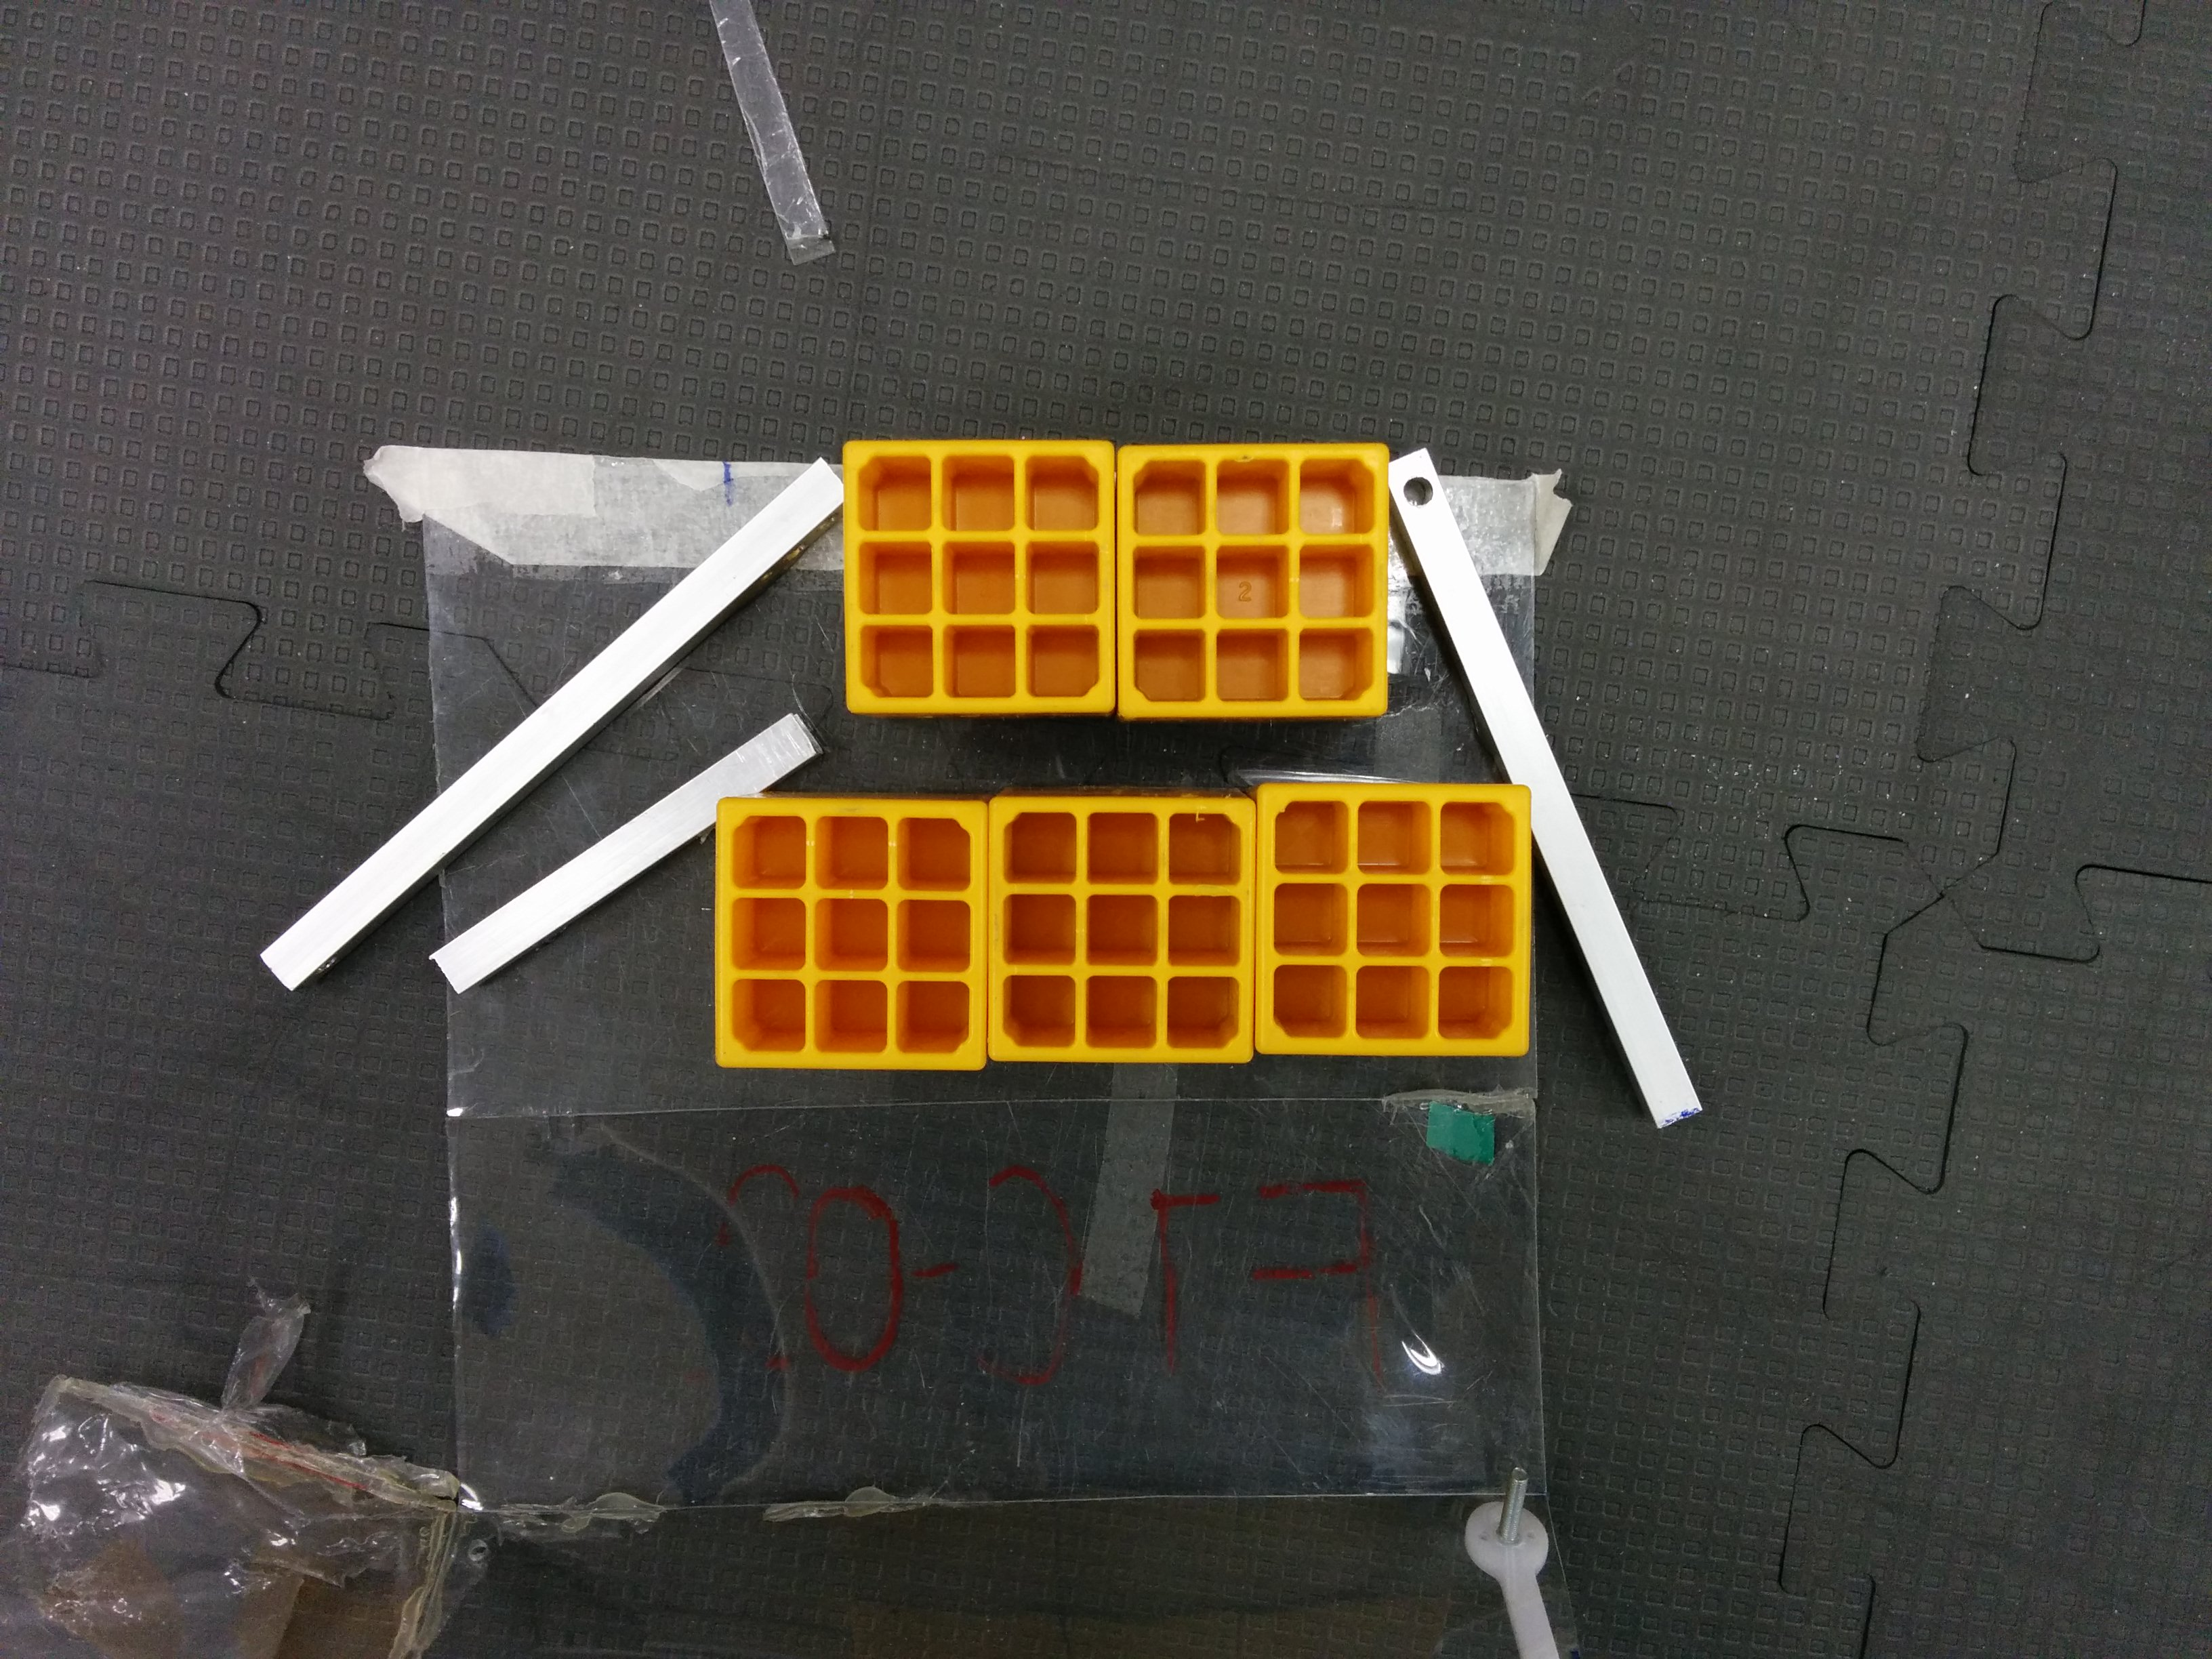
\includegraphics[scale = 0.04]{3Engineering/6Specifications_for_modules/elevator/images/03}}
  		\caption{}
  	\end{minipage}
  	\hfill
  	\begin{minipage}[h]{0.31\linewidth}
  		\center{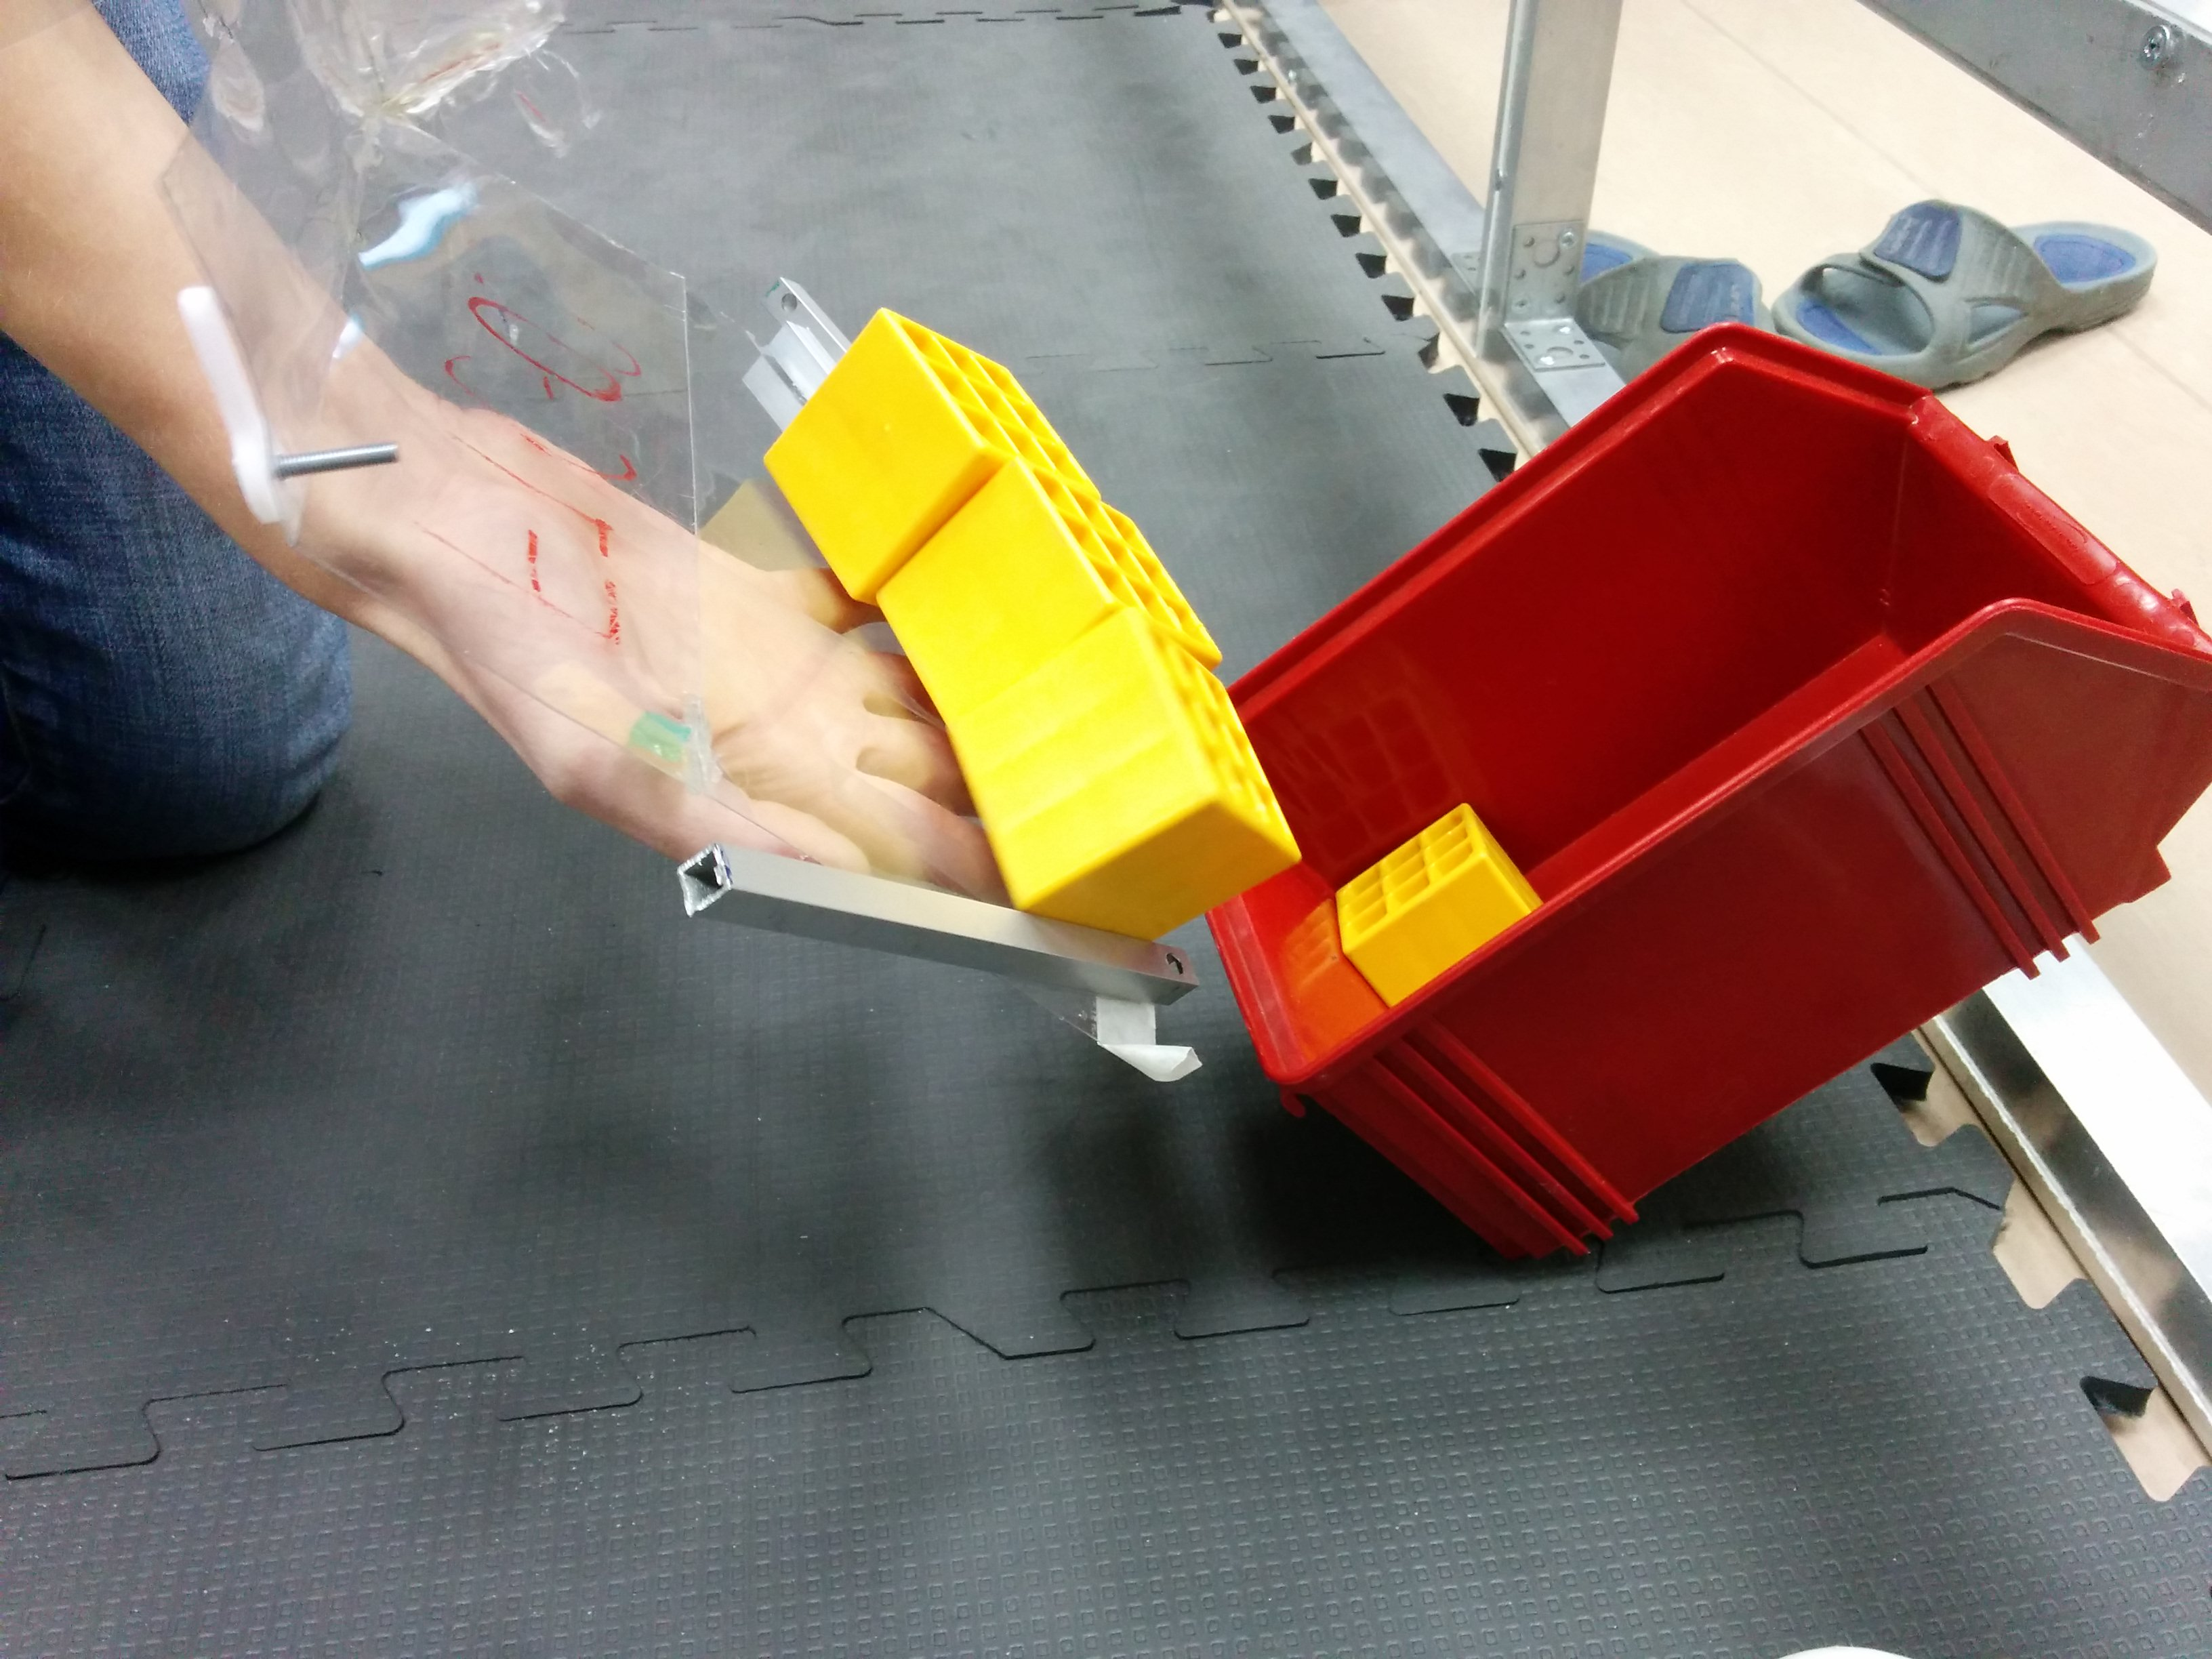
\includegraphics[scale = 0.04]{3Engineering/6Specifications_for_modules/elevator/images/04}}
  		\caption{}
  	\end{minipage}
  	\hfill
  	\begin{minipage}[h]{0.31\linewidth}
  		\center{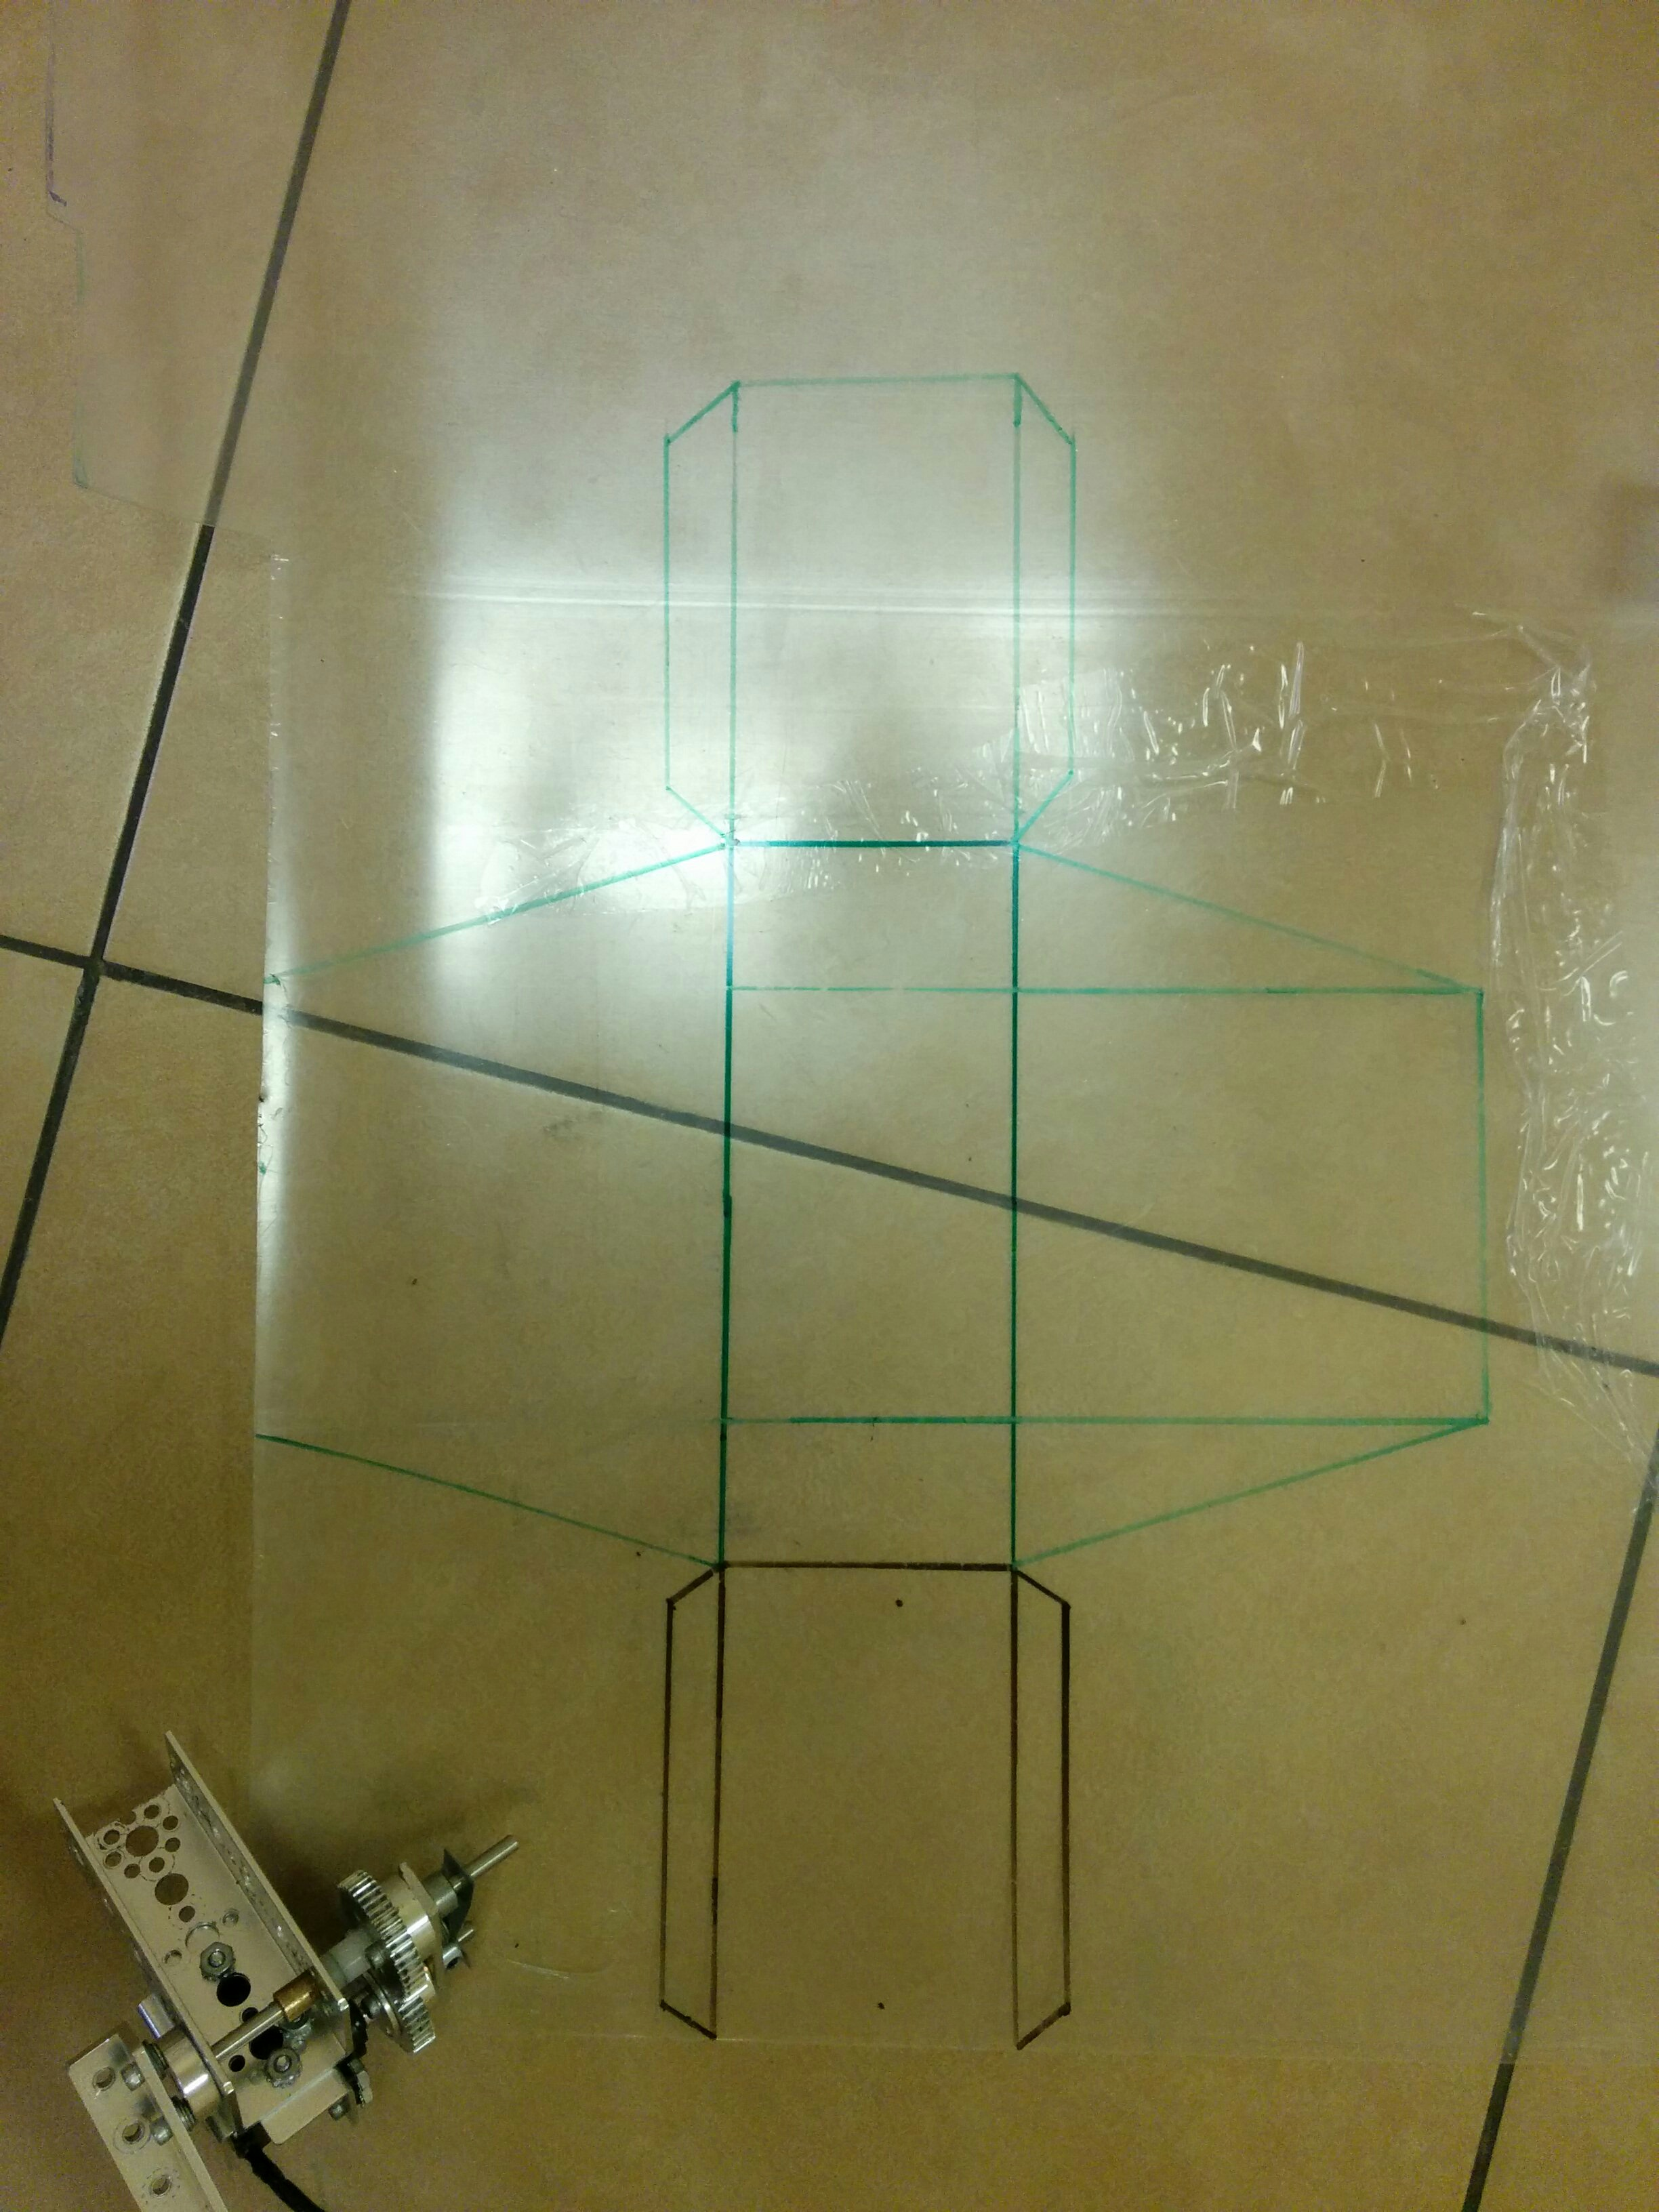
\includegraphics[scale = 0.04]{3Engineering/6Specifications_for_modules/elevator/images/05}}
  		\caption{}
  	\end{minipage}
  \end{figure}

  \item At the 25$^\text{th}$ ) October it was decided to reconsider the concept of the module.

  The reason was that the progress in creating of the module was too low. Firstly, the plastic details for connecting the profiles to each other were not created in material as there was nowhere to make them. Secondly, this system was never made before, so it could have some latent problems. However, first competition was taking place in a week so there was needed a working system.

  According to this, it was decided to find simpler solutions.
  \begin{enumerate*}
  	
  	\item It was decided to use the furniture rails instead of construction profiles because our team had used them in 2 previous FTC seasons and we have an experience in developing the elevator with furniture slats.
  	
  	\item It was decided to not to create the turning mechanism, because it expected to be bulky and difficult in realisation. Instead of it, it was decided to fix the guides in position that allows to score debris into second and high goals. There was no need to change the angle of the elevator for grasping the bar, as the hooks can be delivered to it by additional servo mounted on the top of the lift.
  	
  \end{enumerate*}

  \item In the following week, there was assembled a lifting mechanism. The angle of incline of the guides was $22,5^\circ$. This angle was made using standard holes (without drilling new ones) in TETRIX beams, so the assembly was accurate.

  Each guide was made of 3 furniture slats and surfaces for mounting blocks made of aluminium profiles. Blocks were mounted to these surfaces.

  Next, there was assembled a winch. It was powered by 3 standard TETRIX DC motors. 4 coils were mounted to one axis. The gear ratio on motors was $1:1$ and the diameter of coils was 4 cm, which was enough to pull the robot up: $frac{20 \cdot 3}{2} = 30$ kg (we assume that the robot weighs 10 kg, which is 3 times less).

  \begin{figure}[H]
  	\begin{minipage}[h]{0.31\linewidth}
  		\center{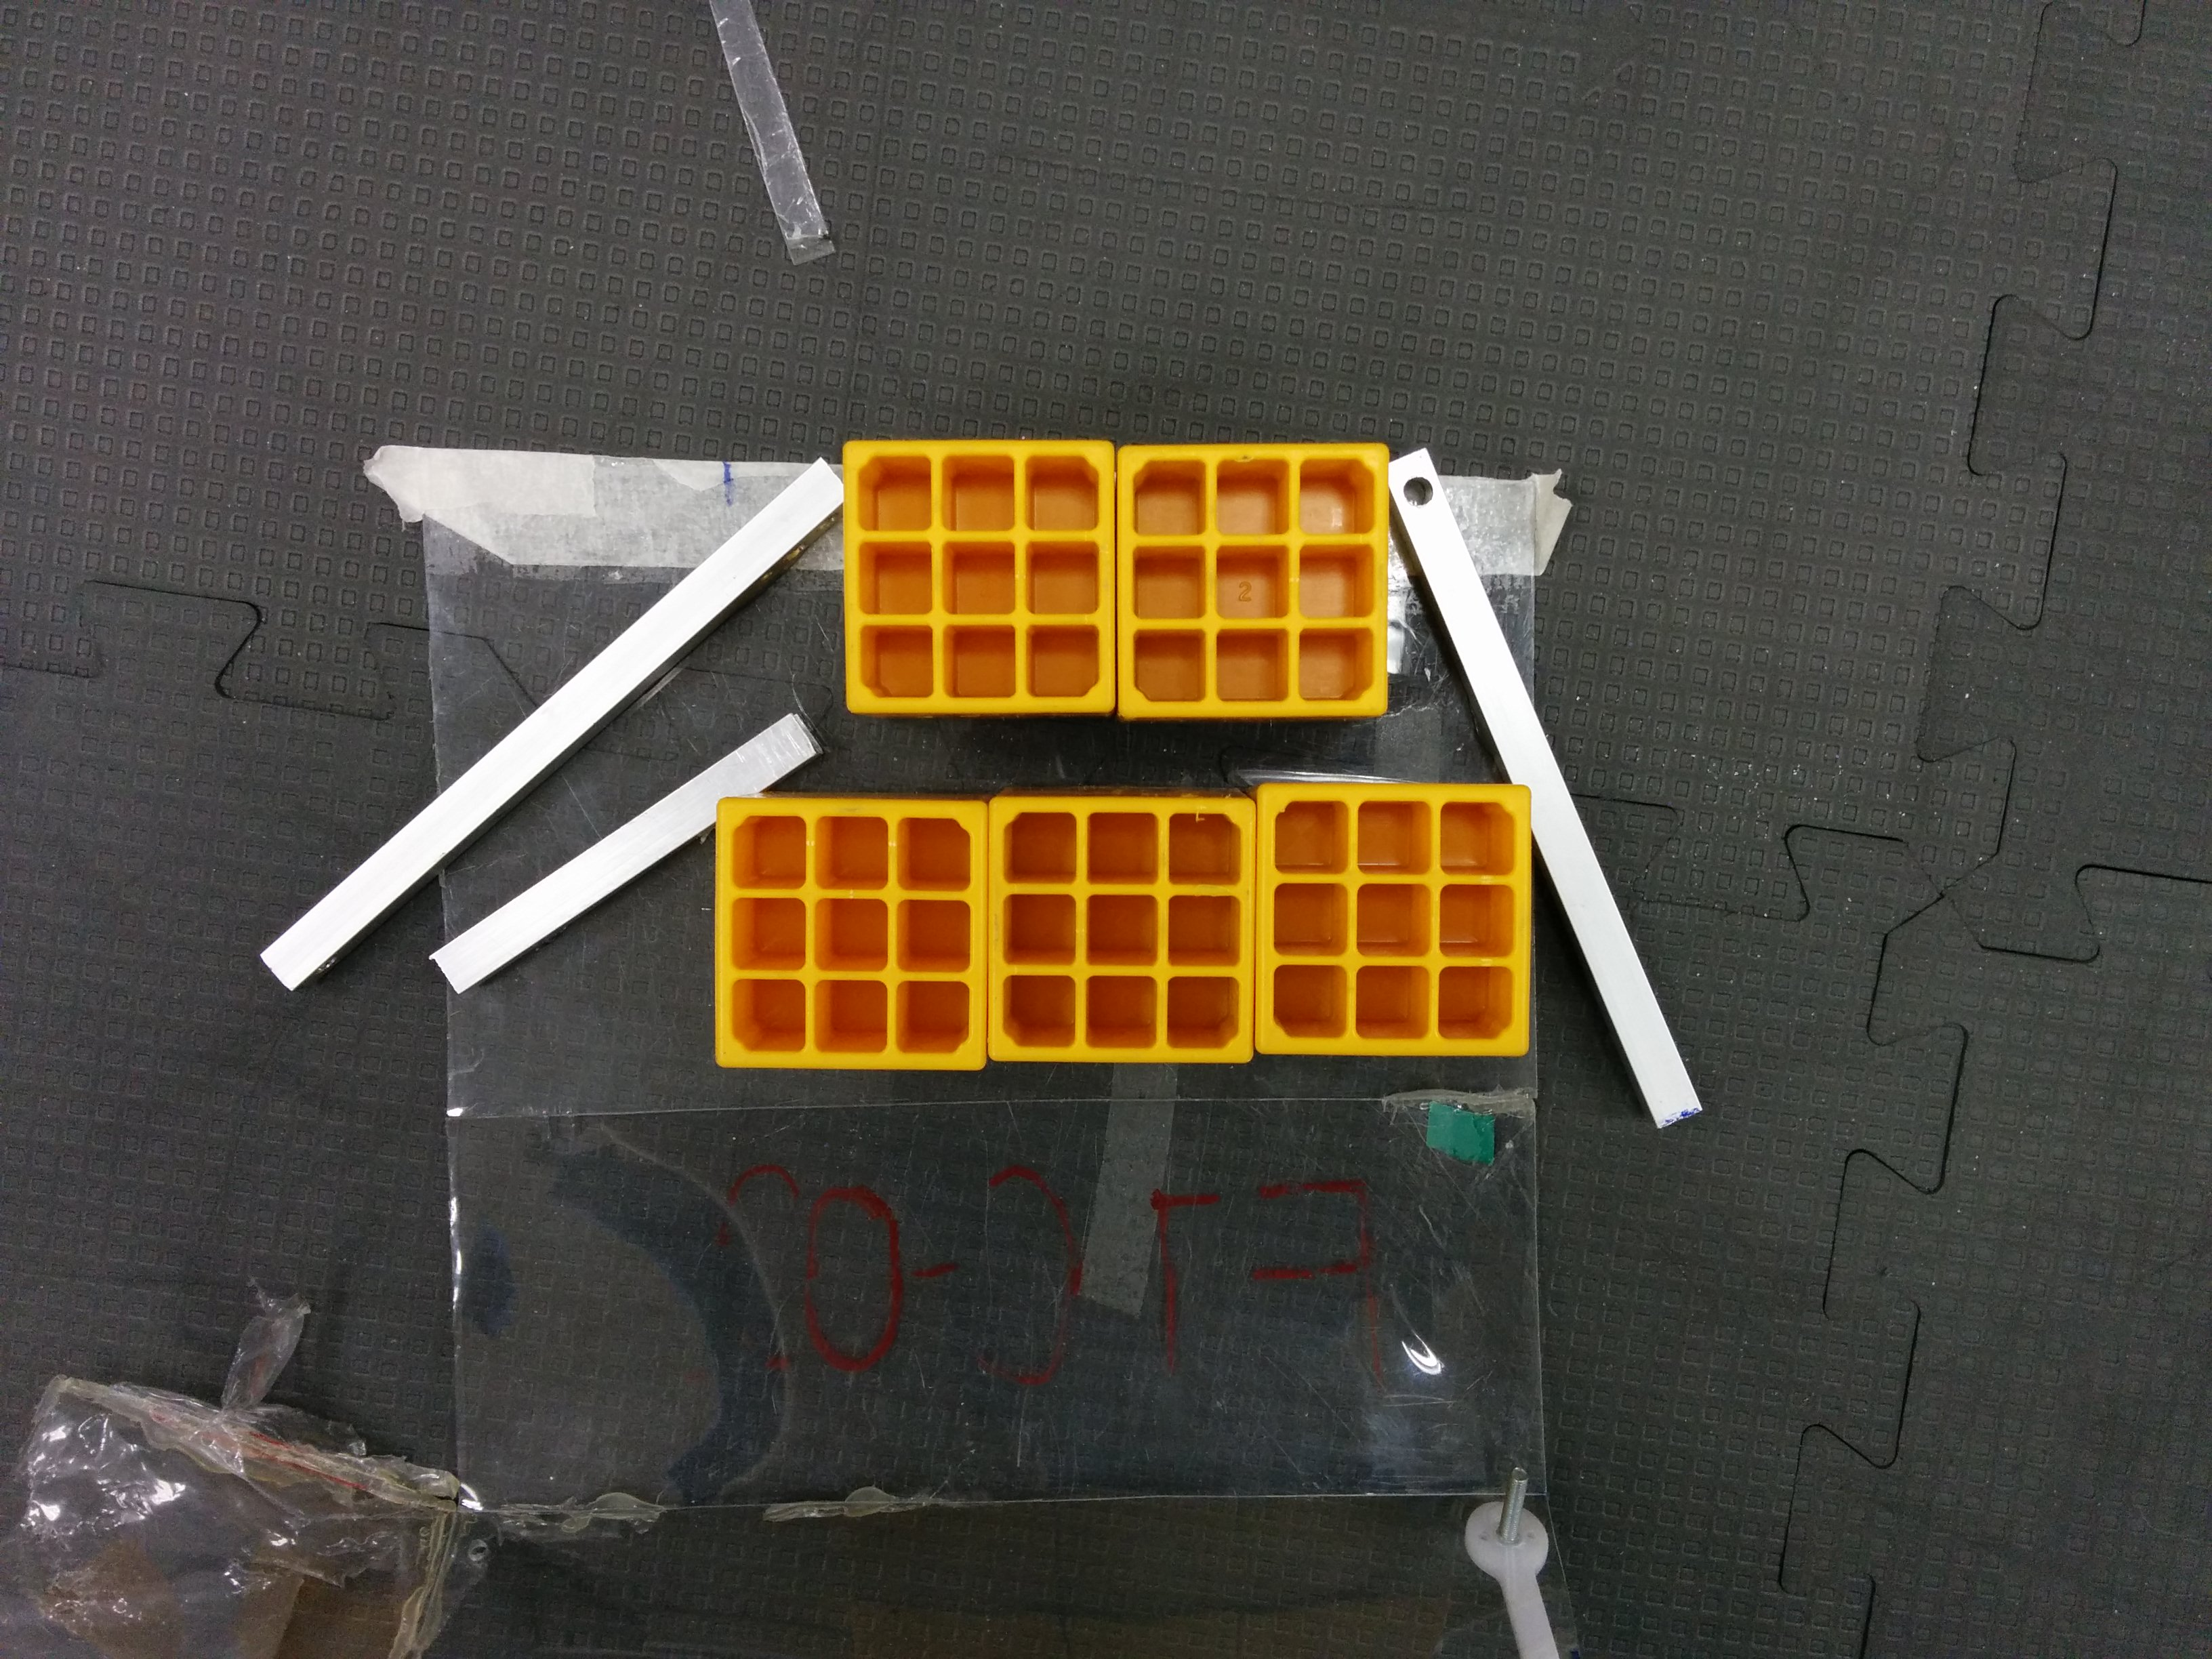
\includegraphics[scale = 0.04]{3Engineering/6Specifications_for_modules/elevator/images/03}}
  		\caption{}
  	\end{minipage}
  	\hfill
  	\begin{minipage}[h]{0.31\linewidth}
  		\center{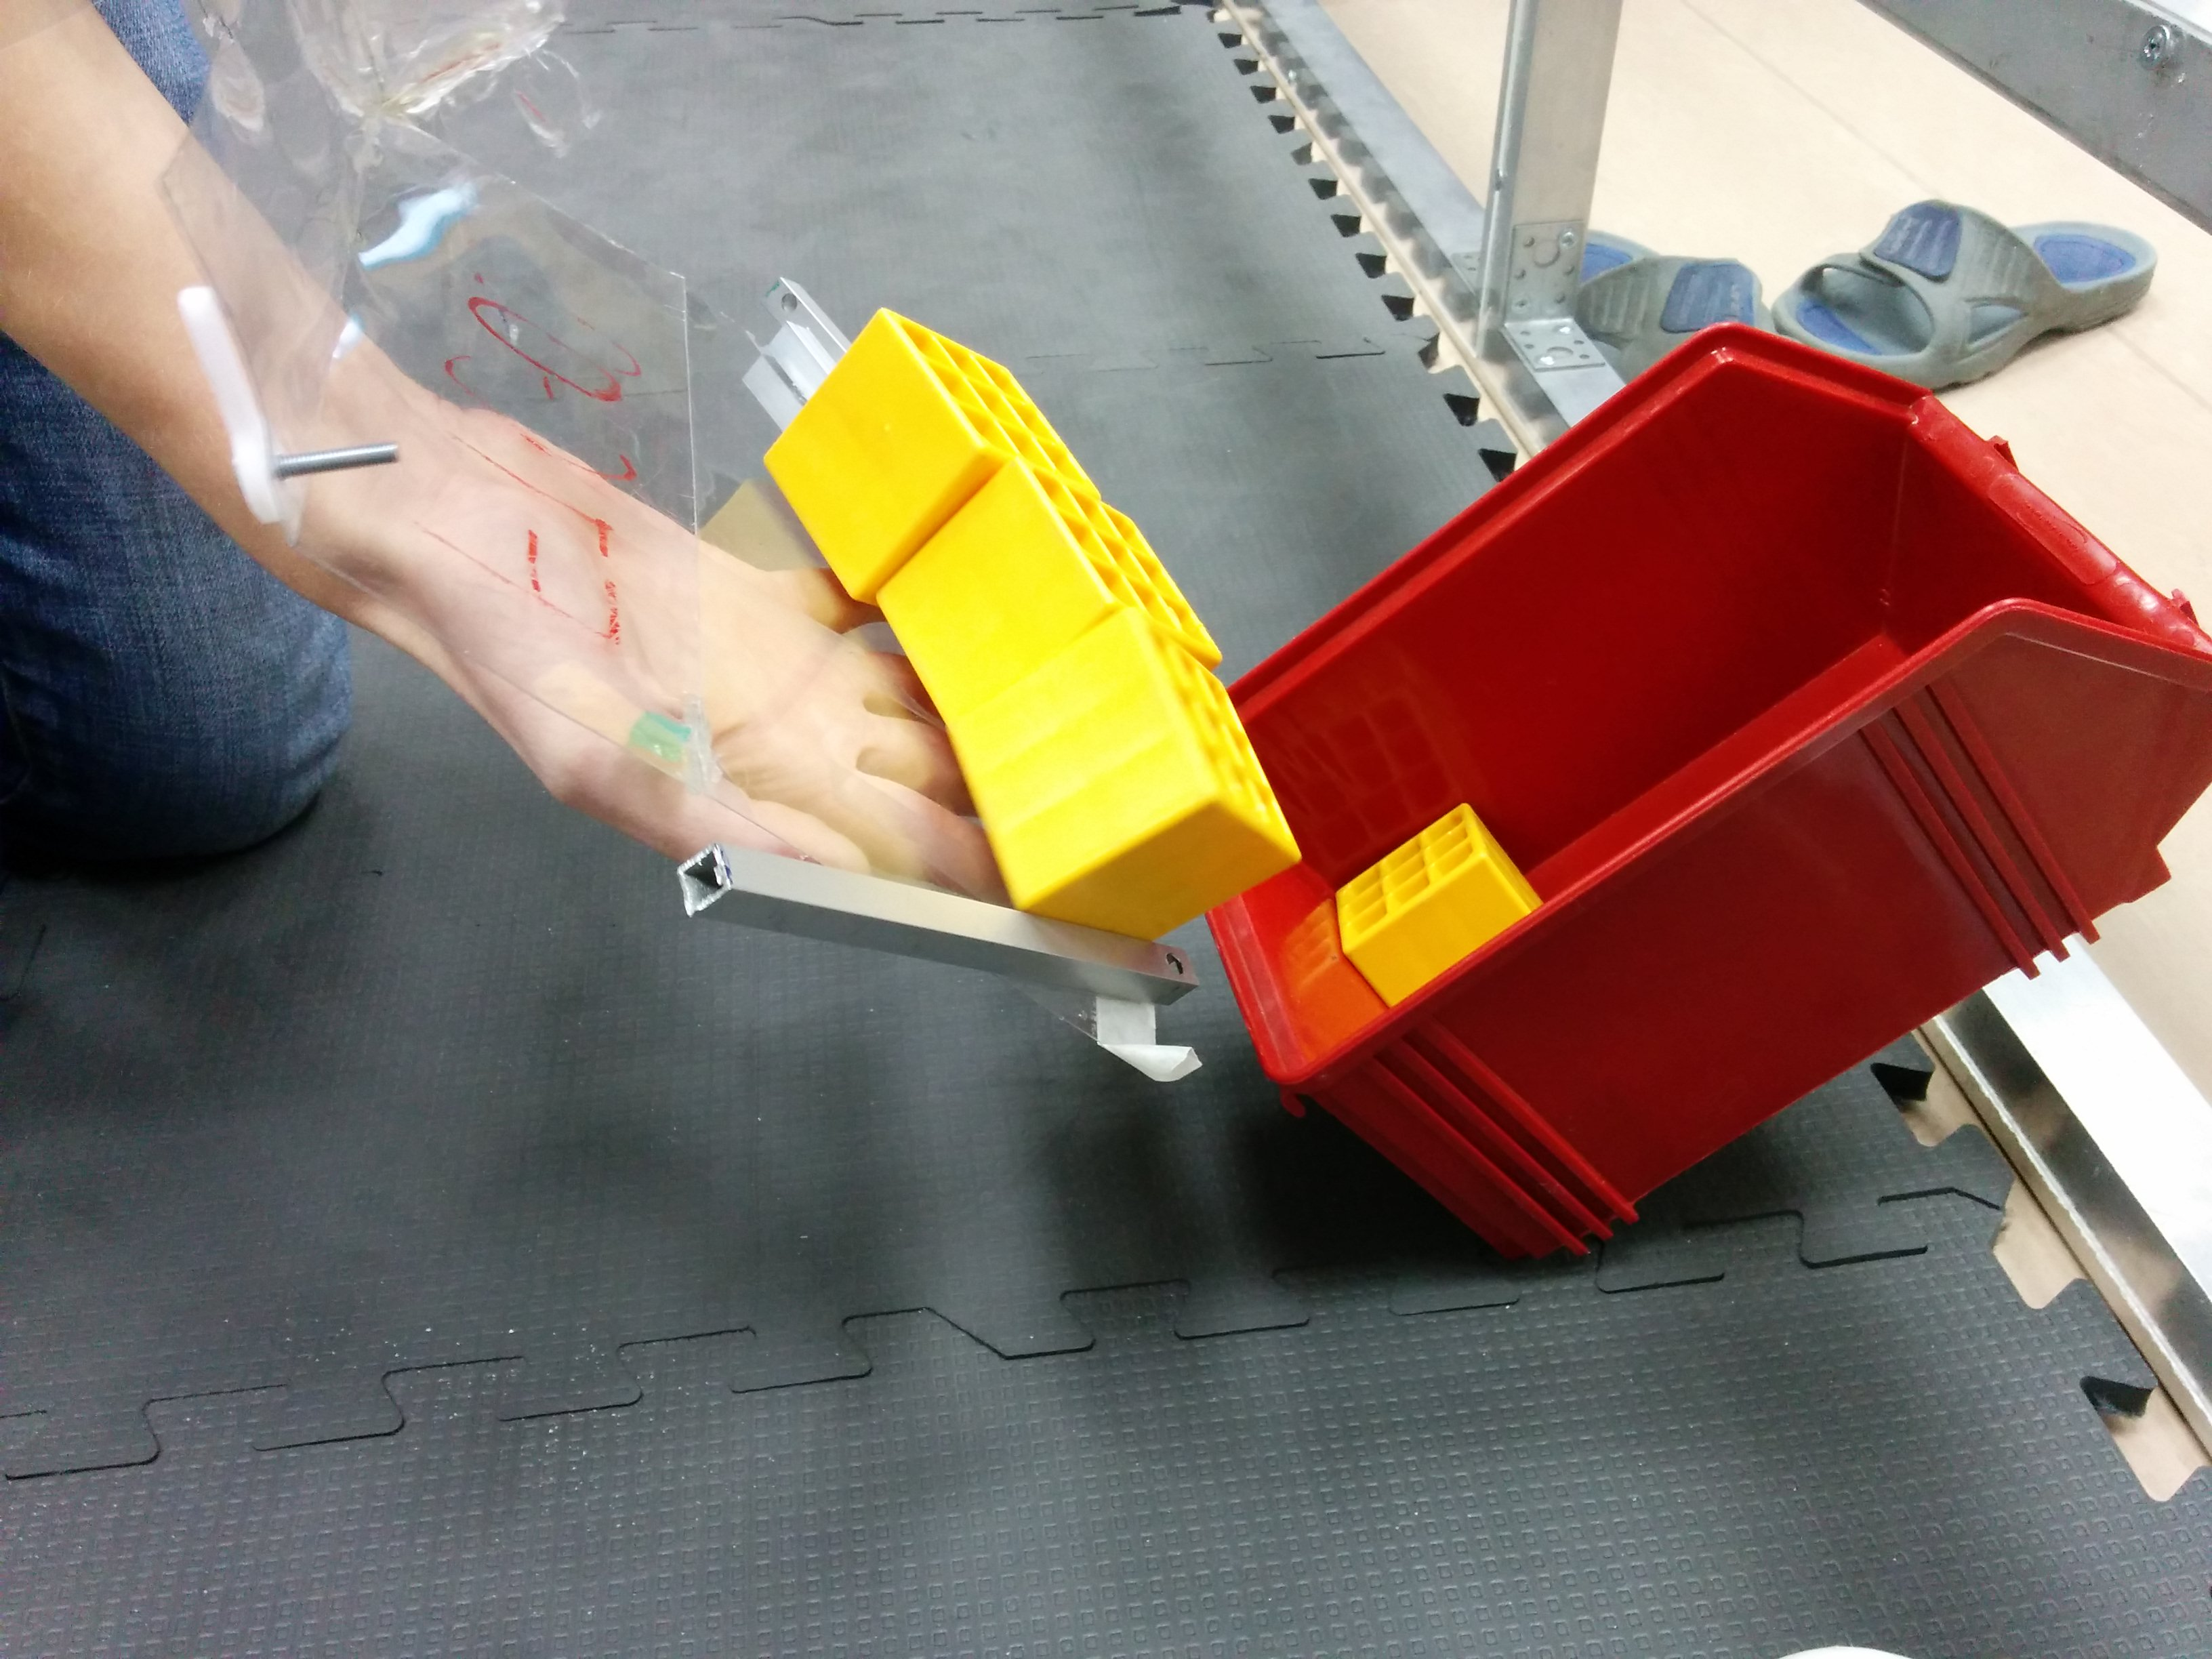
\includegraphics[scale = 0.04]{3Engineering/6Specifications_for_modules/elevator/images/04}}
  		\caption{}
  	\end{minipage}
  	\hfill
  	\begin{minipage}[h]{0.31\linewidth}
  		\center{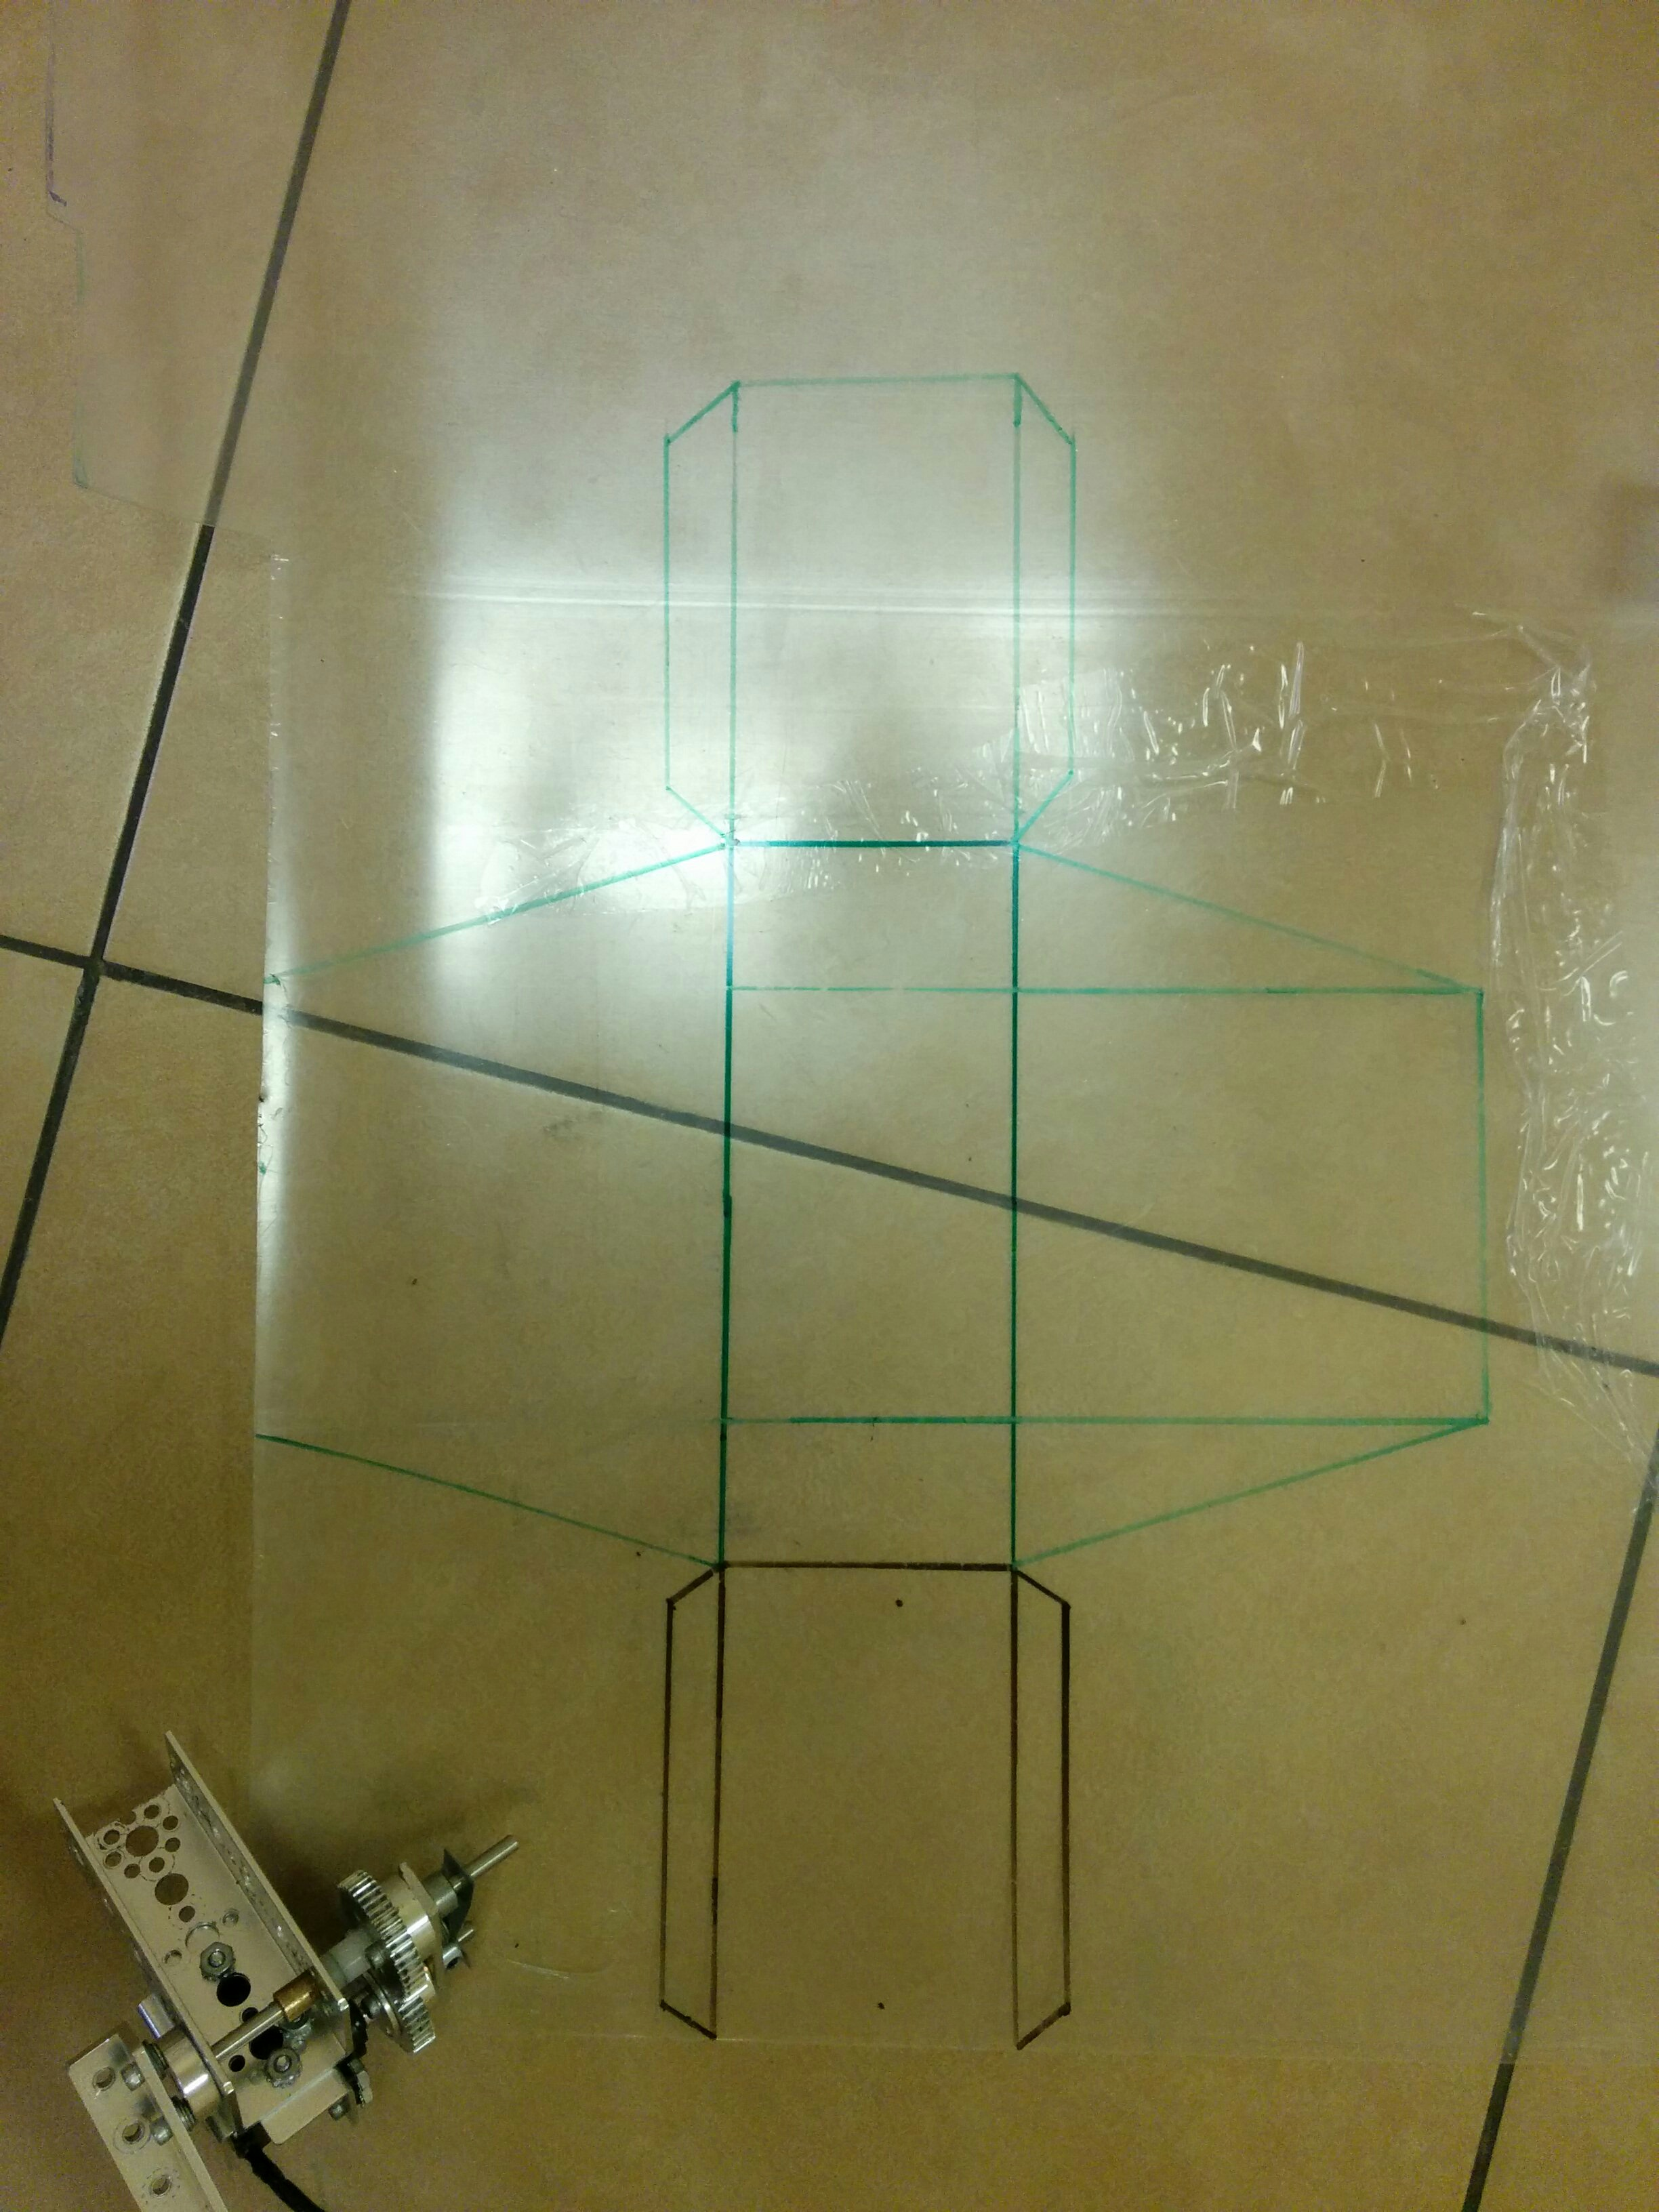
\includegraphics[scale = 0.04]{3Engineering/6Specifications_for_modules/elevator/images/05}}
  		\caption{}
  	\end{minipage}
  \end{figure}

  \item At the 8$^\text{th}$ December there were discussed the results of the competition that took place on 4-5$^\text{th}$ December.
  \begin{enumerate*}
  	
  	\item Firstly, there was a severe mistake in creating of the previous version of the winch. The problem was that the force from motors was transmitted from motors to the coils through the axis. However, the mount of the gear on the axis was not strong enough and broke down. To avoid this problem, it was decided to connect gear to the coils and transmit the force from gear to gear.
  	
  	\item Secondly, it was decided to move guides down for 10 cm in order to lower the center of mass. It was needed to prevent the robot from overturning while climbing the mountain.
  	
  	\item Thirdly, as the concept of the bucket was reshaped, the winch had to be moved to another place. It was decided ti install it above the gripper at the front part of the robot.
  	
  	\item Lastly, it was decided, to stop developing the pull-up option and create a working elevator. If we have time, we can realise pulling up too, but it is not a priority.
  	
  \end{enumerate*}

  \item Then, the guides were moved down and the mount for winch was installed to it's new place.

  \item To discover, what gear ratio is needed on the elevator, there was measured the force, needed to extract the elevator at the ramp. It amounted to 4-5 kg at the each side, which gave us a total of 10 kg.

  It was decided to use caterpillar wheels as coils. The diameter of coils was 5 cm. The optimal solution was to power coils with 2 standard TETRIX DC motors (torque $20 kg \cdot cm$, 2 rounds per second) with gear ratio 1:1. It provided safety coefficient over 1,5: $frac{20 kg \cdot cm \cdot 2}{10 kg \cdot 2,5 cm} = 1.6$. The speed of extracting was $2 rounds / sec \cdot 5 cm \cdot \pi \approx 31,5 cm / sec$, which provided extracting of the elevator to the full in 3,5 seconds.

  \item The winch was installed onto the mount. There also were installed blocks for leading ropes from the elevator to the coils. The mechanism was tested and it was found out that gears were slipping because of not perfect toothing between them. So, it was decided to install a chain transmission instead of gear one.

  \item The elevator was tested in the position, when the robot was standing on the horizontal surface. It was able to entierly extract the elevator in 4.5 seconds, which was a bit more than pre-calculated time of extracting.

  During the testing there were fixed some minor problems.
  \begin{enumerate*}
  	
  	\item Firstly, at one side the cabe was stretched more than at another side. It caused a light bias of the lifting mechanism. This problem was solved by adjustment of the length of cable.
  	
  	\item Secondly, the high load on the blocks pulled mounts of the blocks towards the coils. To avoid the deformation of the beams, there was installed a cross beam, that strethened the construction.
  	
  	\item Another problem is that sometimes ropes can leave the coils. To prevent this, it was decided to make shores for the ropes.
  	
  \end{enumerate*}

  \item After that, the elevator was tested in the position, when the robot was standing on the low zone of the mountain. It was found out, that the power of two TETRIX DC motors is not enough to extract the elevator to the full.

  To solve this problem, it was decided to increas the power of the winch. There were installed 3 NeveRest AndyMark motors instead of 2 standard TETRIX ones. It increased torque 2 times (3 AndyMarks give torque of $3 \cdot 25 = 75kg \cdot cm$, while 2 standard - only $2 \cdot 20 = 40kg \cdot cm$).

  However, it didn't take effect. The power still was not enough to extract the last segment of the lifting mechanism. The principle of extracting the segments of the guides was such that they are extracted one-by-one. So, if there was no friction, the top segment would be extracted before others.

  In fact, the second section (with respect to the bottom) required more power for extraction than the first one and the third section required more power than the second, so the consequence of the extraction was the opposite: the bottom section was going first. According to this, it was concluded, that in the current system there is too much friction.

  To solve the problem, it was decided to hold the cables in another way.

  \begin{figure}[H]
  	\begin{minipage}[h]{1\linewidth}
  		\center{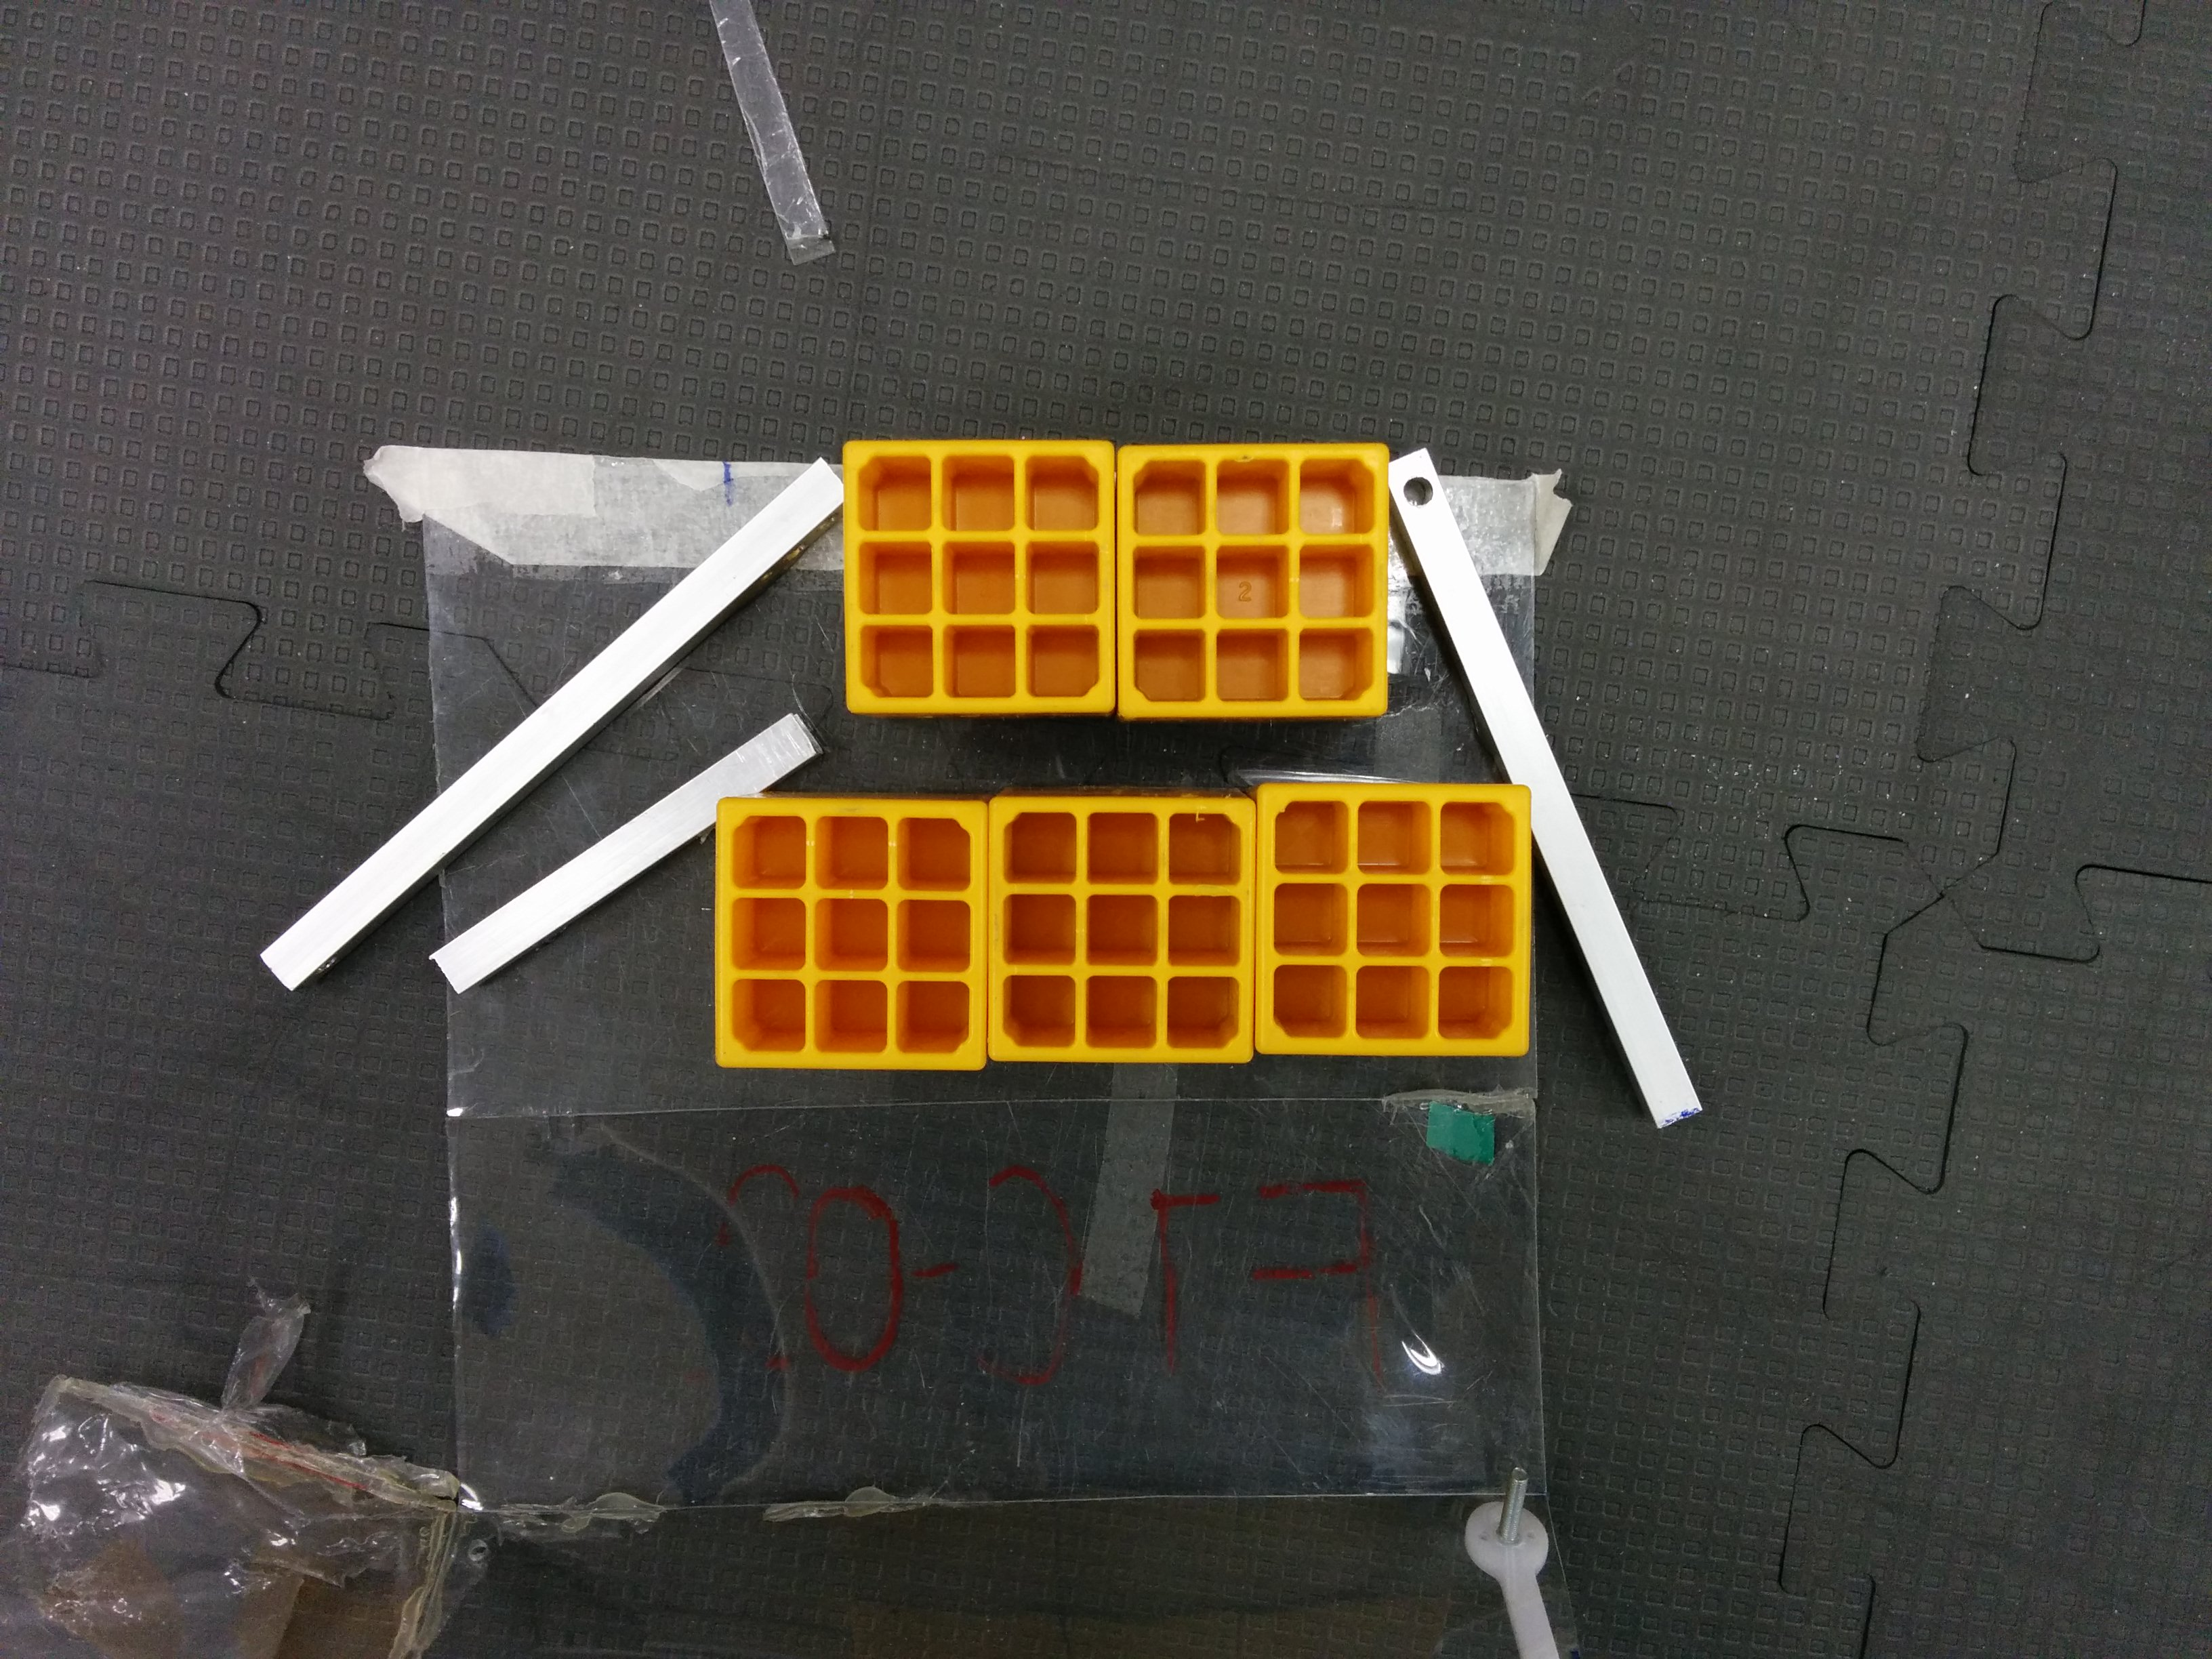
\includegraphics[scale = 0.04]{3Engineering/6Specifications_for_modules/elevator/images/03}}
  		\caption{}
  	\end{minipage}
  \end{figure}

  %The new construction required 3 blocks instead of 5 at a side and the cable from the winch went only through one of them. However, this construction required three times higher torque and three times less length of the cable to reel for extracting. So, the diameter of the coils should be changed correspondingly.

  \item The system of blocks and cables at the lifting mechanism was changed. The coils were also recreated.

  \item The elevator was tested when the robot stood on the mountain. That time it was possible to extract the elevator to the maximal height. However, the ribs that connected pairs of rails together obstructed the movement of the segments.

  That problem occurred because the cables at both sides had different lengths, so each guide was extracting distinctly. But ribs were preventing rails from extracting differently because of inflexible mounts.

  The solution was to make the mount of the rib to one of the rails in a pair flexible. In this construction ribs would still protect the lifting mechanism from bending, but not interfere with it's movement.

  \item After that, there were created flexible mounts for the ribs. These mounts allowed ribs to slide along the axis coincident with the direction od extracting of the lift.




  The winch is a mechanism for extracting of the elevator.

  The concept of the module:

  The winch has two functions: firstly, it extracts the elevator and secondly pulls the robot up. It should have 4 similar coils - 2 for each side of the elevator. All the coils should rotate dependently. It is possible to put them to the one axis. While the first coil reels the elevator's cable and extracts it, the second one releases the cable for pulling up. It is needed because the end of the cable for pulling up is fixed at the top of the elevator. When the coils turn another direction, elevator goes down and the cable for pulling up is being reeled.
  Since the mechanism for grasping the pullup bar connects the cables to the bar, the cable don't contact the elevator anymore. So, when the robot will pull itself up, it won't harm the elevator.

  On the ... There was created an assembly of 3 motors for the winch. The gear ratio was 1:1. The next day it was created the strong axis for coils.

  It was calculated, that to pull the robot up with 3 TETRIX DC motors, the coils should be 4 cm in diameter. The coils were made of plastic pipe. The space between the axis and the pipe was filled with the glued rope. Coils were connected to the axis by the nails. The axis was connected to the motors by the 3-mm screw, put through the hole in the axis.

  On the ... The cables from the elevator were held to the coils and fixed on them.

  When the winch was tested for the first time, it was found out, that there is one weak point: the screw that connected the axis with motors carried too much load, so it broke down as soon as the winch started extracting the elevator. Unfortunately, it was a very severe mistake in development and all the mechanism became useless without the connection between motors and coils.

  Due to this, the mechanism was totally disassembled. After that, it was decided to create a temporary mechanism for extracting of the elevator for the competition "Robofest South", that took place the next day. There were created two undependent coils, powered by one motor each. This construction was also tested, but due to both coils were not synchronised, two sides of the elevator were extracting with different speed and it could break the slats. That's why it was decided to not to use this system at the competition.

  After our team returned from the competition, the problems in all the modules were discussed and the concept of the elevator also changed.
  It was decided, that one mechanism will extract the elevator and another mechanism will pull the robot up. The implementation of the mechanism for extracting the elevator got higher priority.

  Since the construction of the robot was reconsidered, the new place for the winch was above the gripper.


\end{enumerate*}
